\documentclass[a4paper,14pt]{extarticle}

\usepackage[utf8x]{inputenc}
\usepackage[T1,T2A]{fontenc}
\usepackage[russian]{babel}
\usepackage{hyperref}
\usepackage{indentfirst}
\usepackage{here}
\usepackage{array}
\usepackage{graphicx}
\usepackage{caption}
\usepackage{subcaption}
\usepackage{chngcntr}
\usepackage{amsmath}
\usepackage{amssymb}
\usepackage{pgfplots}
\usepackage{pgfplotstable}
\usepackage[left=2cm,right=2cm,top=2cm,bottom=2cm,bindingoffset=0cm]{geometry}
\usepackage{multicol}

\renewcommand{\le}{\ensuremath{\leqslant}}
\renewcommand{\leq}{\ensuremath{\leqslant}}
\renewcommand{\ge}{\ensuremath{\geqslant}}
\renewcommand{\geq}{\ensuremath{\geqslant}}
\renewcommand{\epsilon}{\ensuremath{\varepsilon}}
\renewcommand{\phi}{\ensuremath{\varphi}}

\counterwithin{figure}{section}
\counterwithin{equation}{section}
\counterwithin{table}{section}
\newcommand{\sign}[1][5cm]{\makebox[#1]{\hrulefill}} % Поля подписи и даты
\graphicspath{{pics/}} % Путь до папки с картинками
\captionsetup{justification=centering,margin=1cm}
\def\arraystretch{1.3}

\begin{document}	% начало документа

\begin{titlepage}
\begin{center}
	\textbf{Санкт-Петербургский Политехнический Университет \\Петра Великого}\\[0.3cm]
	\small Институт компьютерных наук и технологий \\[0.3cm]
	\small Кафедра компьютерных систем и программных технологий\\[4cm]
	
	\textbf{ОТЧЕТ}\\ \textbf{о лабораторной работе}\\[0.5cm]
	\textbf{<<Исследование частотных характеристик пассивных RC-цепей>>}\\[0.1cm]
	\textbf{Электротехника и Электроника}\\[10.5cm]
\end{center}

\begin{flushright}
	\begin{minipage}{0.60\textwidth}
		\begin{flushleft}
			\small \textbf{Работу выполнили студенты}\\[3mm]
			\small группа 23501/4 \hspace*{17mm} Дьячков В.В.\\[3mm]
			\small группа 23501/4 \hspace*{17mm} Ламтев А.Ю.\\[5mm]
			
			\small \textbf{Преподаватель}\\[5mm]
		 	\small \sign[3.5cm] \hspace*{8mm} к.т.н., доц. Кочетков Ю.Д.\\[0.5cm]
		\end{flushleft}
	\end{minipage}
\end{flushright}

\vfill

\begin{center}
	\small Санкт-Петербург\\
	\small \the\year
\end{center}
\end{titlepage}


\section{Цель работы}
Исследовать частотные свойства простейших пассивных RC­-цепей и познакомиться с правилами построения частотных характеристик.


\section{Чертеж схемы исследуемого устройства}
\begin{figure}[h]
\centering
\begin{subfigure}[b]{0.34\textwidth}
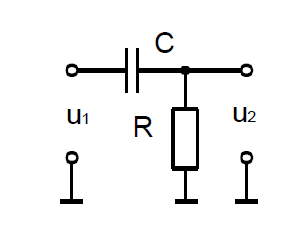
\includegraphics[scale=0.4]{img/a_scheme.png}
\caption{Дифференцирующая\\ цепь}\label{figure:2.1:a}
\end{subfigure}
\begin{subfigure}[b]{0.3\textwidth}
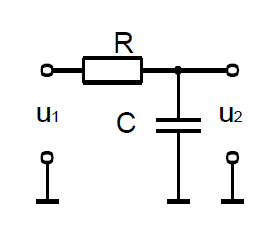
\includegraphics[scale=0.4]{img/b_scheme.png}
\caption{Интегрирующая\\ цепь}\label{figure:2.1:b}
\end{subfigure}
\begin{subfigure}[b]{0.3\textwidth}
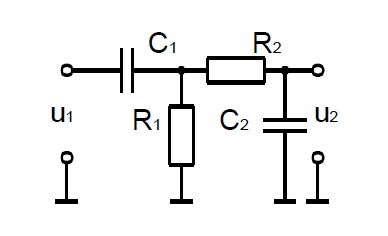
\includegraphics[scale=0.4]{img/v_scheme.png}
\caption{Дифференцирующая и интегрирующая цепь}\label{figure:2.1:c}
\end{subfigure}
\caption{}\label{figure:2.1}
\end{figure}
На рисунке \ref{figure:2.1:a} изображена дифференцирующая RC-цепь, на (\ref{figure:2.1:b}) - интегрирующая RC-цепь, и на  (\ref{figure:2.1:c}) - последоватльное соединение дифференцирующей и интегрирующей RC-­цепей.


\section{Исходные данные}
Исходные значения были подобраны как в таблице \ref{tabular:11}:

\begin{table}[H]
	\begin{center}
	\caption{Исходные данные}
	\def\arraystretch{1.5}
		\begin{tabularx}{\textwidth}{|X|X|}
			\hline
			$R$, кОм & $C$, нФ\\\hline
		     15 & 5\\\hline	
		\end{tabularx}
		\label{tabular:11}
	\end{center}
\end{table}

\section{Теоретические зависимости}
Частота перегиба расчитывается следующим образом:
\begin{equation}
\omega_0 = \frac{1}{RC} = \frac{1}{15 \cdot 10^3 \cdot 5 \cdot 10^{-9}} \simeq 1.334 \cdot 10^4 \hspace*{2mm}
\end{equation}
Отсюда: 
\begin{equation}
f_0 = \frac{\omega_0}{2 \pi} = \frac{1.34}{2\cdot1.341} \simeq 2122.065 (\text{Гц})
\end{equation}

Теоретическая ЛАЧХ для дифференцирующей RC-цепи имеет вид:
\begin{equation}
L_u(\omega) = 20lg \omega RC - 10lg(1+(\omega RC)^2),
\end{equation}

Теоретическая ЛАЧХ для интегрирующей RC-цепи имеет вид:
\begin{equation}
L_u(\omega) = -10lg(1+(\omega RC)^2),
\end{equation}

Теоретическая ЛАЧХ для дифференцирующей и интегрирующей RC-цепи имеет вид:
\begin{equation}
L_u(\omega) = 20lg \omega RC - 10lg(1+7(\omega RC)^2 + (\omega RC)^4).
\end{equation}

При помощи формул 4.3 - 4.5 была сформирована таблица:
\begin{table}[H]
	\begin{center}
	\caption{Значения для построения теоретических ЛАЧХ}
	\def\arraystretch{1.5}
		\begin{tabularx}{\textwidth}{|X|X|X|X|X|}
			\hline
			$f$, Гц & $\omega = 2 \pi f$ & $L_u^1$, дБ & $L_u^2$, дБ & $L_u^3$, дБ\\\hline	
			32 & 201.062 & -36.433 & -0.001 & -36.439\\\hline
			64 & 402.124 & -30.416 & -0.004 & -30.439\\\hline
			128 & 804.248 & -24.407 & -0.016 & -24.500\\\hline
			256 & 1608.495 & -18.433 & -0.063 & -18.793\\\hline
			512 & 3216.991 & -12.596 & -0.246 & -13.845\\\hline
			1024 & 6433.982 & -7.238 & -0.909 & -10.617\\\hline
			2048 & 12867.964 & -3.167 & -2.859 & -9.545\\\hline
			4096 & 25735.927 & -1.033 & -6.745 & -10.412\\\hline
			8192 & 51471.854 & -0.282 & -12.015 & -13.418\\\hline
			16384 & 102943.708 & -0.072 & -17.825 & -18.237\\\hline
			32768 & 205887.416 & -0.018 & -23.792 & -23.900\\\hline
			65536 & 411774.832 & -0.005 & -29.799 & -29.826\\\hline
			131072 & 823549.665 & -0.001 & -35.816 & -35.823\\\hline
			200000 & 1256637.061 & 0.000 & -39.486 & -39.489\\\hline

		\end{tabularx}
		\label{tabular:0}
	\end{center}
\end{table}

\section{Экспериментально снятые зависимости}

В таблицах \ref{tabular:1}, \ref{tabular:2} и \ref{tabular:3} приведены значения входного напряжения, выходного напряжения, коэффициента передачи и коэффициента передачи, выраженного в децибелах, дифференцирующей RC-цепи, для интегрирующей RC-цепи и соединенных последовательно дифференцирующей и интегрирующей RC-цепей соответсвенно. 

%таблицы

\begin{table}[H]
	\begin{center}
	\caption{ЛАЧХ дифференциующей RC-цепи}
	\def\arraystretch{1.5}
		\begin{tabularx}{\textwidth}{|X|X|X|X|X|}
			\hline
			$f$, Гц & $U_{BX}$, В & $U_{BblX}$, В & $K$, В & $20$ · $lg(K)$, дБ\\\hline
			32 & 5.01 & 0.074 & 0.015 & -36.612\\\hline
			64 & 5.05 & 0.151 & 0.030 & -30.486\\\hline
			128 & 5.03 & 0.302 & 0.060 & -24.431\\\hline
			256 & 5.02 & 0.601 & 0.120 & -18.437\\\hline
			512 & 5.03 & 1.133 & 0.225 & -12.947\\\hline
			1024 & 5.00 & 2.130 & 0.426 & -7.412\\\hline
			2048 & 5.01 & 3.380 & 0.675 & -3.418\\\hline
			4096 & 5.00 & 4.260 & 0.852 & -1.391\\\hline
			8192 & 5.03 & 4.660 & 0.926 & -0.664\\\hline
			16384 & 5.02 & 4.750 & 0.946 & -0.480\\\hline
			32768 & 5.00 & 4.780 & 0.956 & -0.391\\\hline
			65536 & 5.01 & 4.780 & 0.954 & -0.408\\\hline
			131072 & 5.02 & 4.790 & 0.954 & -0.407\\\hline
			200000 & 5.03 & 4.800 & 0.954 & -0.407\\\hline	
		\end{tabularx}
		\label{tabular:1}
	\end{center}
\end{table}

\begin{table}[H]
	\begin{center}
	\caption{ЛАЧХ интегрирующей RC-цепи}
	\def\arraystretch{1.5}
		\begin{tabularx}{\textwidth}{|X|X|X|X|X|}
			\hline
			$f$, Гц & $U_{BX}$, В & $U_{BblX}$, В & $K$, В & $20$ · $lg(K)$, дБ\\\hline
			32 & 4.99 & 4.840 & 0.970 & -0.265\\\hline
			64 & 5.00 & 4.840 & 0.968 & -0.282\\\hline
			128 & 5.03 & 4.870 & 0.968 & -0.281\\\hline
			256 & 5.02 & 4.830 & 0.962 & -0.335\\\hline
			512 & 5.03 & 4.720 & 0.938 & -0.553\\\hline
			1024 & 5.02 & 4.320 & 0.861 & -1.304\\\hline
			2048 & 5.03 & 3.430 & 0.682 & -3.325\\\hline
			4096 & 5.02 & 2.170 & 0.432 & -7.285\\\hline
			8192 & 5.00 & 1.170 & 0.234 & -12.616\\\hline
			16384 & 5.02 & 0.596 & 0.119 & -18.509\\\hline
			32768 & 5.02 & 0.299 & 0.060 & -24.501\\\hline
			65536 & 5.03 & 0.150 & 0.030 & -30.510\\\hline
			131072 & 5.01 & 0.075 & 0.015 & -36.496\\\hline
			200000 & 5.01 & 0.049 & 0.010 & -40.193\\\hline			
		\end{tabularx}
		\label{tabular:2}
	\end{center}
\end{table}

\begin{table}[H]
	\begin{center}
	\caption{ЛАЧХ дифференцирующе-интегрирующей RC-цепи}
	\def\arraystretch{1.5}
		\begin{tabularx}{\textwidth}{|X|X|X|X|X|}
			\hline
			$f$, Гц & $U_{BX}$, В & $U_{BblX}$, В & $K$, В & $20$ · $lg(K)$, дБ\\\hline
			32 & 5.02 & 0.076 & 0.015 & -36.364\\\hline
			64 & 5.01 & 0.151 & 0.030 & -30.417\\\hline
			128 & 5.00 & 0.291 & 0.058 & -24.702\\\hline
			256 & 5.01 & 0.562 & 0.112 & -19.002\\\hline
			512 & 5.01 & 0.993 & 0.198 & -14.058\\\hline
			1024 & 5.00 & 1.430 & 0.286 & -10.873\\\hline
			2048 & 5.01 & 1.590 & 0.317 & -9.969\\\hline
			4096 & 5.01 & 1.440 & 0.287 & -10.830\\\hline
			8192 & 4.99 & 1.010 & 0.202 & -13.876\\\hline
			16384 & 5.01 & 0.569 & 0.114 & -18.895\\\hline
			32768 & 5.01 & 0.295 & 0.059 & -24.600\\\hline
			65536 & 5.01 & 0.151 & 0.030 & -30.417\\\hline
			131072 & 5.01 & 0.077 & 0.015 & -36.256\\\hline
			200000 & 5.01 & 0.052 & 0.010 & -39.643\\\hline		
		\end{tabularx}
		\label{tabular:3}
	\end{center}
\end{table}

На рисунках \ref{t:e1}, \ref{t:e2} и \ref{t:e3} приведены теоритические ЛАЧХ, экспериментальные ЛАЧХ и аппроксимирующие прямые для всех цепей.

%рисунки
\setlength{\abovecaptionskip}{0pt}
\setlength{\belowcaptionskip}{-50pt} % чтобы влезло
\begin{figure}[H]
	\begin{center}
		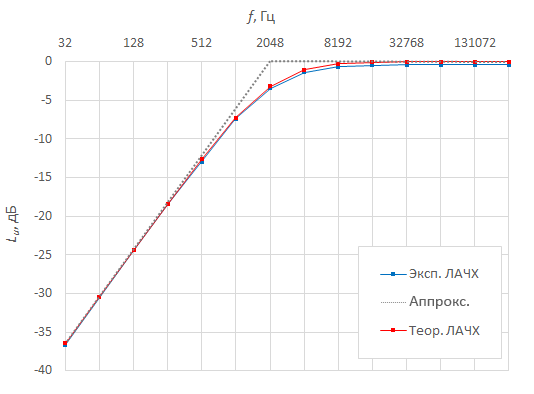
\includegraphics[width=15cm]{img/1}
		\caption{Теоретическая и экспериментальная ЛАЧХ дифференциру-
ющей RC-цепи
} 
		\label{t:e1} % название для ссылок внутри кода
	\end{center}
\end{figure}

\begin{figure}[H]
	\begin{center}
		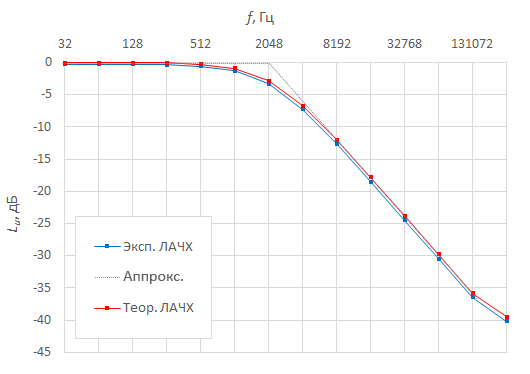
\includegraphics[width=15cm]{img/2}
		\caption{Теоретическая и экспериментальная ЛАЧХ интегрирующей
RC-цепи} 
		\label{t:e2} % название для ссылок внутри кода
	\end{center}
\end{figure}

\setlength{\belowcaptionskip}{0pt} % back to normal
\begin{figure}[H]
	\begin{center}
		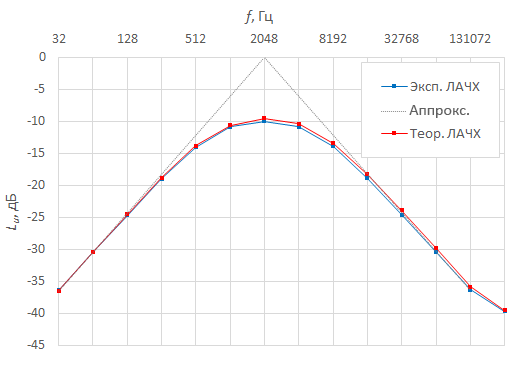
\includegraphics[width=15cm]{img/3}
		\caption{Теоретическая и экспериментальная ЛАЧХ дифференцирующей и интегрирующей RC-цепи} 
		\label{t:e3} % название для ссылок внутри кода
	\end{center}
\end{figure}

\section{Погрешности}

\subsection{Предельно допустимые погрешности}
\begin{center}
$\delta R = 0.1 = 10\%$\\
$\delta C = 0.1 = 10\%$\\
\end{center}

\subsubsection{Дифференцирующей и интегрирующей цепей}

Дифференцирующая и интегрирующая цепи включают в себя по одному резистору и по одному конденсатору, поэтому предельно допустимая относительная погрешность частоты перегиба вычисляется следующим образом:

\begin{equation}
\delta f_0 = \sqrt{(\delta R)^2 + (\delta C)^2} = \sqrt{0.1^2 + 0.1^2} = \sqrt{0.02} = 0.141 = 14.1 \%
\end{equation}

\subsubsection{Дифференцирующе-интегрирующей цепи}

Дифференцирующе-интегрирующая цепь содержит два резистора и два конденсатора, поэтому предельно допустимая относительная погрешность частоты перегиба вычисляется по формуле:

\begin{equation}
\delta f_0 = \sqrt{2 \cdot ((\delta R)^2 + (\delta C)^2)} = \sqrt{2 \cdot (0.1^2 + 0.1^2)} = \sqrt{0.04} = 0.2 = 20 \%
\end{equation}

\subsection{Расчет значения f}
  Необходимо рассчитать значение частоты f, при которой коэффициент передачи равен -3 дБ для дифференцирующей и интегрирующей цепей и -9 дБ для последовательного соединения дифференцирующей и интегрирующей цепей. Построим интерполяционный полином Лагранжа по 3-м точкам (2-й степени), наиболее близким к теоретической $f_0$ = 2122.065 Гц: 1024, 2048 и 4096 Гц.
\subsubsection{Для дифференцирующей RC-цепи}

Для дифференцирующей RC-цепи интерполирующий полином имеет вид:

\begin{equation}
Q_2(x) = (-9.474 \cdot 10^{-7})x^2 + (6.81 \cdot 10^{-3})x -13.393  
\end{equation}

Искомая частота равна f, такому, что $Q_2(f) = -3$:

\begin{equation}
(-9.474 \cdot 10^{-7})f^2 + (6.81 \cdot 10^{-3})f -13.393 = -3
\end{equation}

\begin{equation}
f = 2197.92 (\text{Гц})
\end{equation}

Рассчитаем погрешность для полученного значения f:

\begin{equation}
\delta f = \frac{|f_0 - f|}{f_0} = \frac{|2122.065 - 2197.92|}{2122.065} = 3.57 \% 
\end{equation}

Имеем:\\
$\delta f = 3.57 \% < \delta f_0 = 14.1\%$

\subsubsection{Для интегрирующей RC-цепи}
Для интергрирующей RC-цепи аналогичный интерполяционный полином представим в виде:

\begin{equation}
Q_2(x) = (1.303 \cdot 10^{-8})x^2 - (2.013 \cdot 10^{-3})x + 0.744
\end{equation}

Искомая частота равна f, такому, что $Q_2(f) = -3$:

\begin{equation}
(1.303 \cdot 10^{-8})f^2 - (2.013 \cdot 10^{-3})f + 0.744 = -3
\end{equation}

\begin{equation}
f = 1882.39 (\text{Гц})
\end{equation}

Рассчитаем погрешность для полученного значения f:

\begin{equation}
\delta f = \frac{|f_0 - f|}{f_0} = \frac{|2122.065 - 1882.39|}{2122.065} = 11.3 \% 
\end{equation}

Имеем:\\
$\delta f = 11.3 \% < \delta f_0 = 14.1\%$

\subsubsection{Дифференцирующе-интегрирующая цепь}
Интерполяционный полином дифференцирующе-интегрирующей RC-цепи имеет вид:
\begin{equation}
Q_2(x) = (-4.242 \cdot 10^{-7})x^2 + (2.186 \cdot 10^{-3})x -12.667
\end{equation}
Значение частоты перегиба - это то значение x, при котором 1-ая производная полинома обращается в 0:

\begin{equation}
\frac{d}{dx} (Q_2(x))_{x=f} = 2 \cdot (-4.242 \cdot 10^{-7})f + (2.186 \cdot 10^{-3}) = 0
\end{equation}

\begin{equation}
f = 2576.62 (\text{Гц})
\end{equation}

\begin{equation}
\delta f = \frac{|f_0 - f|}{f_0} = \frac{|2122.065 - 2576.62|}{2122.065} \simeq 20 \% 
\end{equation}

Имеем:\\
$\delta f \simeq 20 \% = \delta f_0 = 20\%$
  
\section{Выводы}
Вычисленные значения частоты перегиба для дифференцирующей, интегрирующей и дифференцирующе-интегрирующей RC-цепей имеют относительную погрешность, которая не превосходит допустимую. Поэтому можно считать, что используемый в лабороторной работе метод определения ЛАЧХ является достаточно точным.
\end{document}
